\hypertarget{the-user-interface-ui-file-and-gtkbuilder}{%
\section{The User Interface (UI) file and
GtkBuilder}\label{the-user-interface-ui-file-and-gtkbuilder}}

\hypertarget{new-open-and-save-button}{%
\subsection{New, Open and Save button}\label{new-open-and-save-button}}

In the last section we made the almost simplest editor possible. It
reads files in the \passthrough{\lstinline!app\_open!} function at
start-up and writes them out when closing the window. It works but is
not very good. It would be better if we had ``New'', ``Open'', ``Save''
and ``Close'' buttons. This section describes how to put those buttons
into the window. Signals and handlers will be explained later.

\begin{figure}
\centering
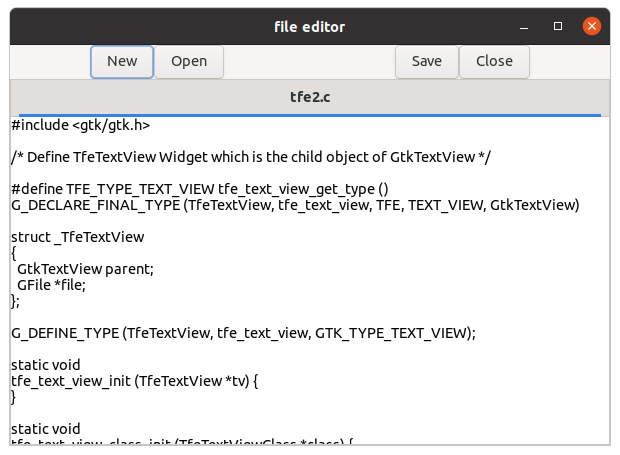
\includegraphics[width=9.3cm,height=6.825cm]{../image/screenshot_tfe2.png}
\caption{Screenshot of the file editor}
\end{figure}

The screenshot above shows the layout. The function
\passthrough{\lstinline!app\_open!} in the source code
\passthrough{\lstinline!tfe2.c!} is as follows.

\begin{lstlisting}[language=C, numbers=left]
static void
app_open (GApplication *app, GFile ** files, gint n_files, gchar *hint, gpointer user_data) {
  GtkWidget *win;
  GtkWidget *nb;
  GtkWidget *lab;
  GtkNotebookPage *nbp;
  GtkWidget *scr;
  GtkWidget *tv;
  GtkTextBuffer *tb;
  char *contents;
  gsize length;
  char *filename;
  int i;

  GtkWidget *boxv;
  GtkWidget *boxh;
  GtkWidget *dmy1;
  GtkWidget *dmy2;
  GtkWidget *dmy3;
  GtkWidget *btnn; /* button for new */
  GtkWidget *btno; /* button for open */
  GtkWidget *btns; /* button for save */
  GtkWidget *btnc; /* button for close */

  win = gtk_application_window_new (GTK_APPLICATION (app));
  gtk_window_set_title (GTK_WINDOW (win), "file editor");
  gtk_window_set_default_size (GTK_WINDOW (win), 600, 400);

  boxv = gtk_box_new (GTK_ORIENTATION_VERTICAL, 0);
  gtk_window_set_child (GTK_WINDOW (win), boxv);

  boxh = gtk_box_new (GTK_ORIENTATION_HORIZONTAL, 0);
  gtk_box_append (GTK_BOX (boxv), boxh);

  dmy1 = gtk_label_new(NULL); /* dummy label for left space */
  gtk_label_set_width_chars (GTK_LABEL (dmy1), 10);
  dmy2 = gtk_label_new(NULL); /* dummy label for center space */
  gtk_widget_set_hexpand (dmy2, TRUE);
  dmy3 = gtk_label_new(NULL); /* dummy label for right space */
  gtk_label_set_width_chars (GTK_LABEL (dmy3), 10);
  btnn = gtk_button_new_with_label ("New");
  btno = gtk_button_new_with_label ("Open");
  btns = gtk_button_new_with_label ("Save");
  btnc = gtk_button_new_with_label ("Close");

  gtk_box_append (GTK_BOX (boxh), dmy1);
  gtk_box_append (GTK_BOX (boxh), btnn);
  gtk_box_append (GTK_BOX (boxh), btno);
  gtk_box_append (GTK_BOX (boxh), dmy2);
  gtk_box_append (GTK_BOX (boxh), btns);
  gtk_box_append (GTK_BOX (boxh), btnc);
  gtk_box_append (GTK_BOX (boxh), dmy3);

  nb = gtk_notebook_new ();
  gtk_widget_set_hexpand (nb, TRUE);
  gtk_widget_set_vexpand (nb, TRUE);
  gtk_box_append (GTK_BOX (boxv), nb);

  for (i = 0; i < n_files; i++) {
    if (g_file_load_contents (files[i], NULL, &contents, &length, NULL, NULL)) {
      scr = gtk_scrolled_window_new ();
      tv = tfe_text_view_new ();
      tb = gtk_text_view_get_buffer (GTK_TEXT_VIEW (tv));
      gtk_text_view_set_wrap_mode (GTK_TEXT_VIEW (tv), GTK_WRAP_WORD_CHAR);
      gtk_scrolled_window_set_child (GTK_SCROLLED_WINDOW (scr), tv);

      tfe_text_view_set_file (TFE_TEXT_VIEW (tv),  g_file_dup (files[i]));
      gtk_text_buffer_set_text (tb, contents, length);
      g_free (contents);
      filename = g_file_get_basename (files[i]);
      lab = gtk_label_new (filename);
      gtk_notebook_append_page (GTK_NOTEBOOK (nb), scr, lab);
      nbp = gtk_notebook_get_page (GTK_NOTEBOOK (nb), scr);
      g_object_set (nbp, "tab-expand", TRUE, NULL);
      g_free (filename);
    } else if ((filename = g_file_get_path (files[i])) != NULL) {
        g_print ("No such file: %s.\n", filename);
        g_free (filename);
    } else
        g_print ("No valid file is given\n");
  }
  if (gtk_notebook_get_n_pages (GTK_NOTEBOOK (nb)) > 0) {
    gtk_widget_show (win);
  } else
    gtk_window_destroy (GTK_WINDOW (win));
}
\end{lstlisting}

The aim is to build the widgets of the main application window.

\begin{itemize}
\tightlist
\item
  25-27: Creates a GtkApplicationWindow instance and sets the title and
  default size.
\item
  29-30: Creates a GtkBox instance \passthrough{\lstinline!boxv!}. It is
  a vertical box and a child of GtkApplicationWindow. It has two
  children. The first child is a horizontal box. The second child is a
  GtkNotebook.
\item
  32-33: Creates a GtkBox instance \passthrough{\lstinline!boxh!} and
  appends it to \passthrough{\lstinline!boxv!} as a first child.
\item
  35-40: Creates three dummy labels. The labels
  \passthrough{\lstinline!dmy1!} and \passthrough{\lstinline!dmy3!} has
  a character width of ten. The other label
  \passthrough{\lstinline!dmy2!} has hexpand property which is set to be
  TRUE. This makes the label expands horizontally as long as possible.
\item
  41-44: Creates four buttons.
\item
  46-52: Appends these GtkLabel and GtkButton to
  \passthrough{\lstinline!boxh!}.
\item
  54-57: Creates a GtkNotebook instance and sets hexpand and vexpand
  properties TRUE. This makes it expand horizontally and vertically as
  big as possible. It is appended to \passthrough{\lstinline!boxv!} as
  the second child.
\end{itemize}

The number of lines to build the widgets is 33(=57-25+1). We also needed
many additional variables (\passthrough{\lstinline!boxv!},
\passthrough{\lstinline!boxh!}, \passthrough{\lstinline!dmy1!}, \ldots),
most of which weren't necessary, except for building the widgets. Are
there any good solution to reduce these work?

Gtk provides GtkBuilder. It reads user interface (UI) data and builds a
window. It reduces this cumbersome work.

\hypertarget{the-ui-file}{%
\subsection{The UI File}\label{the-ui-file}}

First, let's look at the UI file \passthrough{\lstinline!tfe3.ui!} that
is used to define the widget structure.

\begin{lstlisting}[language=XML, numbers=left]
<?xml version="1.0" encoding="UTF-8"?>
<interface>
  <object class="GtkApplicationWindow" id="win">
    <property name="title">file editor</property>
    <property name="default-width">600</property>
    <property name="default-height">400</property>
    <child>
      <object class="GtkBox" id="boxv">
        <property name="orientation">GTK_ORIENTATION_VERTICAL</property>
        <child>
          <object class="GtkBox" id="boxh">
            <property name="orientation">GTK_ORIENTATION_HORIZONTAL</property>
            <child>
              <object class="GtkLabel" id="dmy1">
                <property name="width-chars">10</property>
              </object>
            </child>
            <child>
              <object class="GtkButton" id="btnn">
                <property name="label">New</property>
              </object>
            </child>
            <child>
              <object class="GtkButton" id="btno">
                <property name="label">Open</property>
              </object>
            </child>
            <child>
              <object class="GtkLabel" id="dmy2">
                <property name="hexpand">TRUE</property>
              </object>
            </child>
            <child>
              <object class="GtkButton" id="btns">
                <property name="label">Save</property>
              </object>
            </child>
            <child>
              <object class="GtkButton" id="btnc">
                <property name="label">Close</property>
              </object>
            </child>
            <child>
              <object class="GtkLabel" id="dmy3">
                <property name="width-chars">10</property>
              </object>
            </child>
          </object>
        </child>
        <child>
          <object class="GtkNotebook" id="nb">
            <property name="hexpand">TRUE</property>
            <property name="vexpand">TRUE</property>
          </object>
        </child>
      </object>
    </child>
  </object>
</interface>
\end{lstlisting}

The structure of this file is XML. Constructs that begin with
\passthrough{\lstinline!<!} and end with \passthrough{\lstinline!>!} are
called tags. There are two types of tags, the start tag and the end tag.
For example, \passthrough{\lstinline!<interface>!} is a start tag and
\passthrough{\lstinline!</interface>!} is an end tag. The UI file begins
and ends with interface tags. Some tags, for example object tags, can
have a class and id attributes in their start tag.

\begin{itemize}
\tightlist
\item
  1: The first line is XML declaration. It specifies that the version of
  XML is 1.0 and the encoding is UTF-8. Even if the line is left out,
  GtkBuilder builds objects from the ui file. But ui files must use
  UTF-8 encoding, or GtkBuilder can't recognize it and a fatal error
  occurs.
\item
  3-6: An object with \passthrough{\lstinline!GtkApplicationWindow!}
  class and \passthrough{\lstinline!win!} id is defined. This is the top
  level window. And the three properties of the window are defined.
  \passthrough{\lstinline!title!} property is ``file editor'',
  \passthrough{\lstinline!default-width!} property is 600 and
  \passthrough{\lstinline!default-height!} property is 400.
\item
  7: child tag means a child of the widget above. For example, line 7
  tells us that GtkBox object which id is ``boxv'' is a child widget of
  \passthrough{\lstinline!win!}.
\end{itemize}

Compare this ui file and the lines 25-57 in the source code of
\passthrough{\lstinline!app\_open!} function. Those two describe the
same structure of widgets.

You can check the ui file with
\passthrough{\lstinline!gtk4-builder-tool!}.

\begin{itemize}
\tightlist
\item
  \passthrough{\lstinline!gtk4-builder-tool validate <ui file name>!}
  validates the ui file. If the ui file includes some syntactical error,
  \passthrough{\lstinline!gtk4-builder-tool!} prints the error.
\item
  \passthrough{\lstinline!gtk4-builder-tool simplify <ui file name>!}
  simplifies the ui file and prints the result. If
  \passthrough{\lstinline!--replace!} option is given, it replaces the
  ui file with the simplified one. If the ui file specifies a value of
  property but it is default, then it will be removed. And some values
  are simplified. For example, ``TRUE''and ``FALSE'' becomes ``1'' and
  ``0'' respectively. However, ``TRUE'' or ``FALSE'' is better for
  maintenance.
\end{itemize}

It is a good idea to check your ui file before compiling.

\hypertarget{gtkbuilder}{%
\subsection{GtkBuilder}\label{gtkbuilder}}

GtkBuilder builds widgets based on the ui file.

\begin{lstlisting}[language=C]
GtkBuilder *build;

build = gtk_builder_new_from_file ("tfe3.ui");
win = GTK_WIDGET (gtk_builder_get_object (build, "win"));
gtk_window_set_application (GTK_WINDOW (win), GTK_APPLICATION (app));
nb = GTK_WIDGET (gtk_builder_get_object (build, "nb"));
\end{lstlisting}

The function \passthrough{\lstinline!gtk\_builder\_new\_from\_file!}
reads the file given as an argument. Then, it builds the widgets and
creates GtkBuilder object. The function
\passthrough{\lstinline!gtk\_builder\_get\_object (build, "win")!}
returns the pointer to the widget \passthrough{\lstinline!win!}, which
is the id in the ui file. All the widgets are connected based on the
parent-children relationship described in the ui file. We only need
\passthrough{\lstinline!win!} and \passthrough{\lstinline!nb!} for the
program after this, so we don't need to take out any other widgets. This
reduces lines in the C source file.

\begin{lstlisting}
$ cd tfe; diff tfe2.c tfe3.c
58a59
>   GtkBuilder *build;
60,103c61,65
<   GtkWidget *boxv;
<   GtkWidget *boxh;
<   GtkWidget *dmy1;
<   GtkWidget *dmy2;
<   GtkWidget *dmy3;
<   GtkWidget *btnn; /* button for new */
<   GtkWidget *btno; /* button for open */
<   GtkWidget *btns; /* button for save */
<   GtkWidget *btnc; /* button for close */
< 
<   win = gtk_application_window_new (GTK_APPLICATION (app));
<   gtk_window_set_title (GTK_WINDOW (win), "file editor");
<   gtk_window_set_default_size (GTK_WINDOW (win), 600, 400);
< 
<   boxv = gtk_box_new (GTK_ORIENTATION_VERTICAL, 0);
<   gtk_window_set_child (GTK_WINDOW (win), boxv);
< 
<   boxh = gtk_box_new (GTK_ORIENTATION_HORIZONTAL, 0);
<   gtk_box_append (GTK_BOX (boxv), boxh);
< 
<   dmy1 = gtk_label_new(NULL); /* dummy label for left space */
<   gtk_label_set_width_chars (GTK_LABEL (dmy1), 10);
<   dmy2 = gtk_label_new(NULL); /* dummy label for center space */
<   gtk_widget_set_hexpand (dmy2, TRUE);
<   dmy3 = gtk_label_new(NULL); /* dummy label for right space */
<   gtk_label_set_width_chars (GTK_LABEL (dmy3), 10);
<   btnn = gtk_button_new_with_label ("New");
<   btno = gtk_button_new_with_label ("Open");
<   btns = gtk_button_new_with_label ("Save");
<   btnc = gtk_button_new_with_label ("Close");
< 
<   gtk_box_append (GTK_BOX (boxh), dmy1);
<   gtk_box_append (GTK_BOX (boxh), btnn);
<   gtk_box_append (GTK_BOX (boxh), btno);
<   gtk_box_append (GTK_BOX (boxh), dmy2);
<   gtk_box_append (GTK_BOX (boxh), btns);
<   gtk_box_append (GTK_BOX (boxh), btnc);
<   gtk_box_append (GTK_BOX (boxh), dmy3);
< 
<   nb = gtk_notebook_new ();
<   gtk_widget_set_hexpand (nb, TRUE);
<   gtk_widget_set_vexpand (nb, TRUE);
<   gtk_box_append (GTK_BOX (boxv), nb);
< 
---
>   build = gtk_builder_new_from_file ("tfe3.ui");
>   win = GTK_WIDGET (gtk_builder_get_object (build, "win"));
>   gtk_window_set_application (GTK_WINDOW (win), GTK_APPLICATION (app));
>   nb = GTK_WIDGET (gtk_builder_get_object (build, "nb"));
>   g_object_unref(build);
138c100
<   app = gtk_application_new ("com.github.ToshioCP.tfe2", G_APPLICATION_HANDLES_OPEN);
---
>   app = gtk_application_new ("com.github.ToshioCP.tfe3", G_APPLICATION_HANDLES_OPEN);
\end{lstlisting}

\passthrough{\lstinline!60,103c61,65!} means 44 (=103-60+1) lines are
changed to 5 (=65-61+1) lines. Therefore, 39 lines are reduced. Using ui
file not only shortens C source files, but also makes the widgets'
structure clear.

Now I'll show you \passthrough{\lstinline!app\_open!} function in the C
file \passthrough{\lstinline!tfe3.c!}.

\begin{lstlisting}[language=C, numbers=left]
static void
app_open (GApplication *app, GFile ** files, gint n_files, gchar *hint, gpointer user_data) {
  GtkWidget *win;
  GtkWidget *nb;
  GtkWidget *lab;
  GtkNotebookPage *nbp;
  GtkWidget *scr;
  GtkWidget *tv;
  GtkTextBuffer *tb;
  char *contents;
  gsize length;
  char *filename;
  int i;
  GtkBuilder *build;

  build = gtk_builder_new_from_file ("tfe3.ui");
  win = GTK_WIDGET (gtk_builder_get_object (build, "win"));
  gtk_window_set_application (GTK_WINDOW (win), GTK_APPLICATION (app));
  nb = GTK_WIDGET (gtk_builder_get_object (build, "nb"));
  g_object_unref(build);
  for (i = 0; i < n_files; i++) {
    if (g_file_load_contents (files[i], NULL, &contents, &length, NULL, NULL)) {
      scr = gtk_scrolled_window_new ();
      tv = tfe_text_view_new ();
      tb = gtk_text_view_get_buffer (GTK_TEXT_VIEW (tv));
      gtk_text_view_set_wrap_mode (GTK_TEXT_VIEW (tv), GTK_WRAP_WORD_CHAR);
      gtk_scrolled_window_set_child (GTK_SCROLLED_WINDOW (scr), tv);

      tfe_text_view_set_file (TFE_TEXT_VIEW (tv),  g_file_dup (files[i]));
      gtk_text_buffer_set_text (tb, contents, length);
      g_free (contents);
      filename = g_file_get_basename (files[i]);
      lab = gtk_label_new (filename);
      gtk_notebook_append_page (GTK_NOTEBOOK (nb), scr, lab);
      nbp = gtk_notebook_get_page (GTK_NOTEBOOK (nb), scr);
      g_object_set (nbp, "tab-expand", TRUE, NULL);
      g_free (filename);
    } else if ((filename = g_file_get_path (files[i])) != NULL) {
        g_print ("No such file: %s.\n", filename);
        g_free (filename);
    } else
        g_print ("No valid file is given\n");
  }
  if (gtk_notebook_get_n_pages (GTK_NOTEBOOK (nb)) > 0) {
    gtk_widget_show (win);
  } else
    gtk_window_destroy (GTK_WINDOW (win));
}
\end{lstlisting}

The whole source code of \passthrough{\lstinline!tfe3.c!} is stored in
src/tfe directory. If you want to see it, click the link above.

\hypertarget{using-ui-string}{%
\subsubsection{Using ui string}\label{using-ui-string}}

GtkBuilder can build widgets using string. Use the function
\passthrough{\lstinline!gtk\_builder\_new\_from\_string!} instead of
\passthrough{\lstinline!gtk\_builder\_new\_from\_file!}.

\begin{lstlisting}[language=C]
char *uistring;

uistring =
"<interface>"
  "<object class="GtkApplicationWindow" id="win">"
    "<property name=\"title\">file editor</property>"
    "<property name=\"default-width\">600</property>"
    "<property name=\"default-height\">400</property>"
    "<child>"
      "<object class=\"GtkBox\" id=\"boxv\">"
        "<property name="orientation">GTK_ORIENTATION_VERTICAL</property>"
... ... ...
... ... ...
"</interface>";

build = gtk_builder_new_from_stringfile (uistring);
\end{lstlisting}

This method has an advantage and disadvantage. The advantage is that the
ui string is written in the source code. So ui file is not necessary on
runtime. The disadvantage is that writing C string is a bit bothersome
because of the double quotes. If you want to use this method, you should
write a script that transforms ui file into C-string.

\begin{itemize}
\tightlist
\item
  Add backslash before each double quote.
\item
  Add double quotes at the left and right of the string in each line.
\end{itemize}

\hypertarget{using-gresource}{%
\subsubsection{Using Gresource}\label{using-gresource}}

Using Gresource is similar to using string. But Gresource is compressed
binary data, not text data. And there's a compiler that compiles ui file
into Gresource. It can compile not only text files but also binary files
such as images, sounds and so on. And after compilation, it bundles them
up into one Gresource object.

An xml file is necessary for the resource compiler
\passthrough{\lstinline!glib-compile-resources!}. It describes resource
files.

\begin{lstlisting}[language=XML, numbers=left]
<?xml version="1.0" encoding="UTF-8"?>
<gresources>
  <gresource prefix="/com/github/ToshioCP/tfe3">
    <file>tfe3.ui</file>
  </gresource>
</gresources>
\end{lstlisting}

\begin{itemize}
\tightlist
\item
  2: \passthrough{\lstinline!gresources!} tag can include multiple
  gresources (gresource tags). However, this xml has only one gresource.
\item
  3: The gresource has a prefix
  \passthrough{\lstinline!/com/github/ToshioCP/tfe3!}.
\item
  4: The gresource has \passthrough{\lstinline!tfe3.ui!}. And it is
  pointed by \passthrough{\lstinline!/com/github/ToshioCP/tfe3/tfe3.ui!}
  because it needs prefix. If you want to add more files, then insert
  them between line 4 and 5.
\end{itemize}

Save this xml text to \passthrough{\lstinline!tfe3.gresource.xml!}. The
gresource compiler \passthrough{\lstinline!glib-compile-resources!}
shows its usage with the argument \passthrough{\lstinline!--help!}.

\begin{lstlisting}
$ LANG=C glib-compile-resources --help
Usage:
  glib-compile-resources [OPTION?] FILE

Compile a resource specification into a resource file.
Resource specification files have the extension .gresource.xml,
and the resource file have the extension called .gresource.

Help Options:
  -h, --help                   Show help options

Application Options:
  --version                    Show program version and exit
  --target=FILE                Name of the output file
  --sourcedir=DIRECTORY        The directories to load files referenced in FILE from (default: current directory)
  --generate                   Generate output in the format selected for by the target filename extension
  --generate-header            Generate source header
  --generate-source            Generate source code used to link in the resource file into your code
  --generate-dependencies      Generate dependency list
  --dependency-file=FILE       Name of the dependency file to generate
  --generate-phony-targets     Include phony targets in the generated dependency file
  --manual-register            Don?t automatically create and register resource
  --internal                   Don?t export functions; declare them G_GNUC_INTERNAL
  --external-data              Don?t embed resource data in the C file; assume it's linked externally instead
  --c-name                     C identifier name used for the generated source code
  -C, --compiler               The target C compiler (default: the CC environment variable)
\end{lstlisting}

Now run the compiler.

\begin{lstlisting}
$ glib-compile-resources tfe3.gresource.xml --target=resources.c --generate-source
\end{lstlisting}

Then a C source file \passthrough{\lstinline!resources.c!} is generated.
Modify \passthrough{\lstinline!tfe3.c!} and save it as
\passthrough{\lstinline!tfe3\_r.c!}.

\begin{lstlisting}[language=C]
#include "resources.c"
... ... ...
... ... ...
build = gtk_builder_new_from_resource ("/com/github/ToshioCP/tfe3/tfe3.ui");
... ... ...
... ... ...
\end{lstlisting}

Then, compile and run it. The window appears and it is the same as the
screenshot at the beginning of this page.
